\section{Auswertung}
\label{sec:Auswertung}

\subsection{Detektorscan}

Für den Detektorscan wird ein Gaußfit der Form

\begin{equation*}
    I(\alpha) = \frac{a}{\sqrt{2\pi\sigma^2}} \exp{-\frac{(x-\mu)^2}{2\sigma^2}} + b
\end{equation*}

gemacht und die Halbwertsbreite sowie die maximale Intensität berechnet, zu sehen in \autoref{fig:detektorscan}.

\begin{figure}[H]
    \centering
    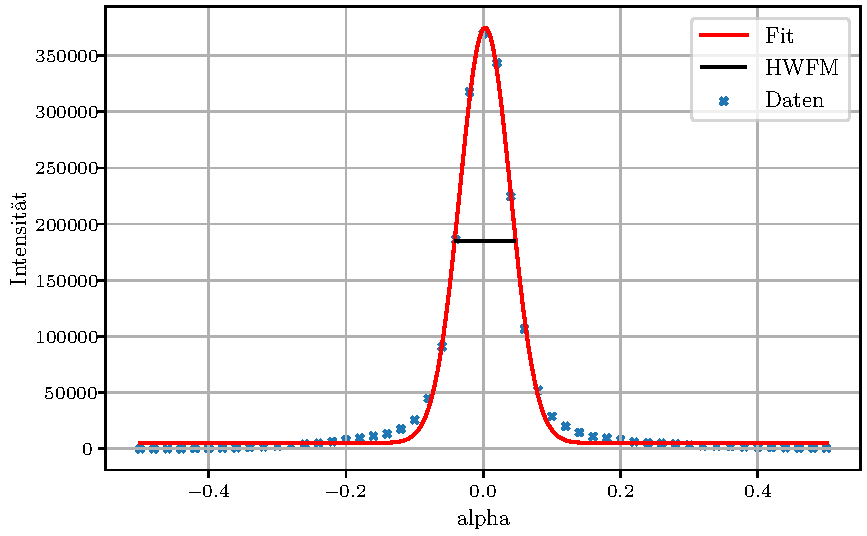
\includegraphics[width=\textwidth]{plots/detectorscan.pdf}
    \caption{Detektorscan mit Gaußfit und HWFM-Linie.}
    \label{fig:detektorscan}
\end{figure}

Die Fitparameter berechnen sich zu

\begin{align*}
    \mu &= \qty{0.0026(4)}{\degree} \\
    \sigma &= \qty{0.0369(4)}{\degree} \\
    a &= \num{34247(410)} \\
    b &= \num{5197(917)}.
\end{align*}

Das Maximum befindet sich bei ungefähr
\begin{equation*}
    I_\text{max} = \num{369567(329)}
\end{equation*}
und die Grenzen der vollen Breite bei halbem Maximum (FWHM) liegen bei ungefähr
\begin{align*}
   \text{HWFM}_\text{links} &= \qty{-0.041}{\degree} \\
   \text{HWFM}_\text{rechts} &= \qty{0.046}{\degree}.
\end{align*}

\subsection{Geometrie des Strahls}

Die Strahlbreite wird über den Z-Scan ermittelt, zu sehen in \autoref{fig:strahlbreite}.

\begin{figure}[H]
    \centering
    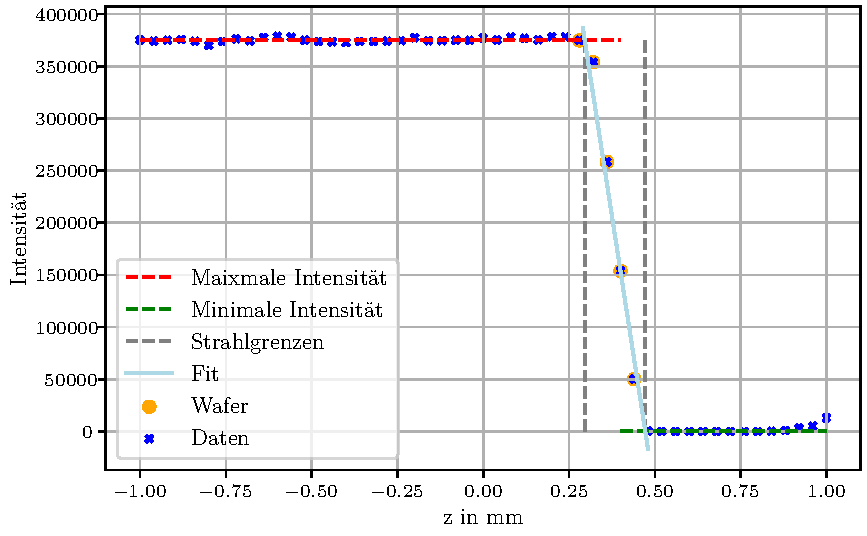
\includegraphics[width=\textwidth]{plots/zscan.pdf}
    \caption{Z-Scan des Strahls. Die volle Intensität, wenn der Strahl nicht geblockt wird, und die minimale Intensität, wenn der Strahl komplett geblockt ist, sind über Mittelwerte dargestellt.
    Die Intensitätsabnahme des Strahls wird linear genähert und die Grenzen markiert.}
    \label{fig:strahlbreite}
\end{figure}

Die Intensitäten werden genähert mit
\begin{align*}
    I_\text{volle Intensität} &= \qty{374812(344)}{} \\
    I_\text{minimale Intensität} &= \qty{399(23)}{} \\
    I_\text{Strahl}(\alpha) &= \qty{-2123867(241153)}{\per\degree} \cdot \alpha + \qty{1002844(87880)}{}.
\end{align*}

Die Lasergrenzen liegen somit bei
\begin{align*}
    \alpha_\text{Linke Grenze} &= \qty{0.295(18)}{\milli\meter} \\
    \alpha_\text{Rechte Grenze} &= \qty{0.471(25)}{\milli\meter},
\end{align*}

was einer Strahlbreite von 
\begin{equation*}
    d = \qty{0.176(30)}{\milli\meter}
\end{equation*}

entspricht. 

Der Geometriewinkel wird einmal berechnet und anschließend gemessen. Nach %%%%% REF GEOMETRIEWINKEL 
ergibt sich mit der Strahlbreite $d$ ein theoretischer Geometriewinkel von
\begin{equation*}
    \alpha_\text{g, theo.} = \qty{0.51(9)}{\degree}.
\end{equation*}

Mit dem Rockingscan in \autoref{fig:rockingscan} kann der Geometriewinkel gemessen werden.

\begin{figure}[H]
    \centering
    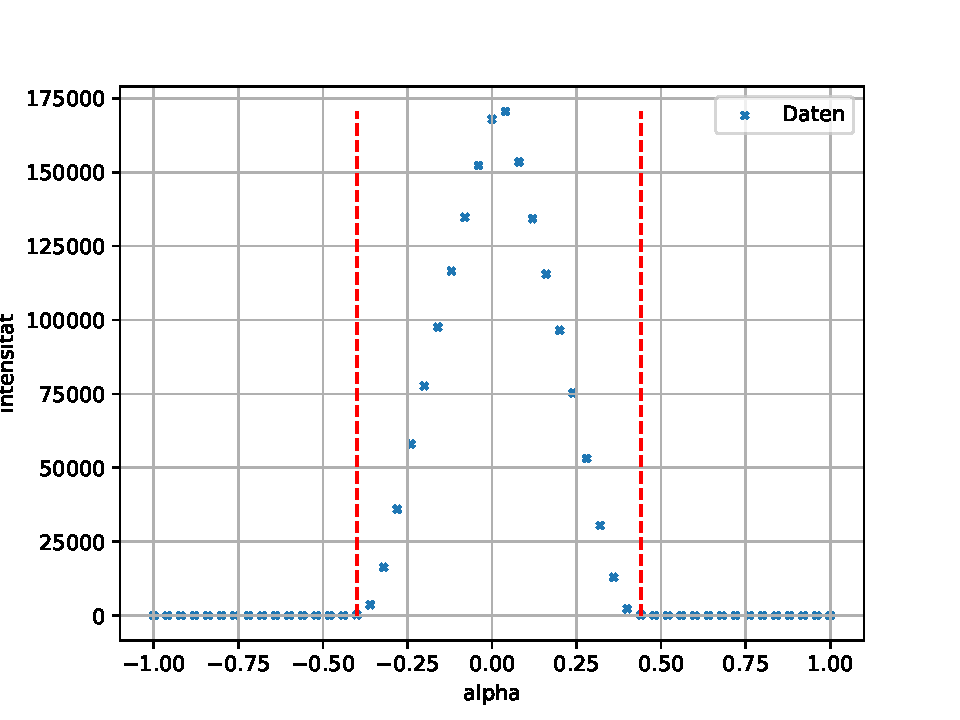
\includegraphics[width=\textwidth]{plots/rockingscan.pdf}
    \caption{Rockingscan zur Bestimmung des Geometriewinkels, angedeutet mit gestrichelten Linien.}
    \label{fig:rockingscan}
\end{figure}

Die Nulldurchgänge liegen hier bei $\alpha_{0\text{, links}} = \qty{-0.4}{\degree}$ und $\alpha_{0\text{, rechts}} = \qty{0.44}{\degree}$.
Der mittlere Geometriewinkel liegt in der Messung bei 
\begin{equation*}
    \alpha_\text{g, mess.} = \qty{0.42(2)}{\degree}
\end{equation*}